\documentclass[10pt]{beamer}
\usepackage[utf8]{inputenc}
\usepackage[T1]{fontenc}

% Include SIunits to get \unit for unit typesetting
\usepackage[squaren]{SIunits}
% Set the math mode font to sans-serif
\let\mathrm\mathsf

% Enable rounded corners for standard blocks:
% \setbeamertemplate{blocks}[rounded]

\title{Example Template}
\date{2014-06-18}
\author[Johannes Agricola]{Johannes Agricola}

\usetheme{ugoe}

\def\insertlogos{%
  
\includegraphics[height=1.3cm]{logos/BMBF-Gef-Logo.pdf}%
  \hspace{1cm}%
  
\includegraphics[height=1.3cm]{logos/FSP101-Atlas-Logo.pdf}%
  \hspace{1cm}%
  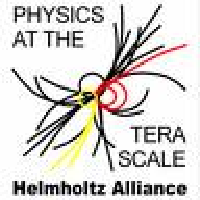
\includegraphics[height=1.3cm]{logos/helmholtz_logo.pdf}%
  \hspace{1cm}%
  
\includegraphics[height=1.3cm]{logos/logo3.pdf}%
}

\begin{document}

\begin{frame}
  \titlepage
\end{frame}

\begin{frame}
  \frametitle{Test Slide}

  \begin{itemize}
    \item 
      Some example text
      \begin{itemize}
        \item 
          And some subitems
      \end{itemize}
  \end{itemize}
\end{frame}

\begin{frame}
  \frametitle{Test slide with a slightly longer frame title}

  \begin{itemize}
    \item 
      Long frame titles should not be used. 
    \item
      Nevertheless, they are possible now.
  \end{itemize}
\end{frame}
\begin{frame}
  \frametitle{Shorter Title}
  \framesubtitle{And a slightly longer subtitle.}

  \begin{itemize}
    \item 
      Long frame titles should not be used. 
    \item
      Nevertheless, they are possible now.
  \end{itemize}
\end{frame}

\begin{frame}{Some Blocks\ldots}
  \begin{block}{Standard Blocks}
    \textbackslash{}begin\{block\}\ldots
  \end{block}
  \begin{alertblock}{Alerted Blocks}
    \textbackslash{}begin\{alertblock\}\ldots
  \end{alertblock}
  \begin{exampleblock}{Example Blocks}
    \textbackslash{}begin\{exampleblock\}\ldots
  \end{exampleblock}
\end{frame}

\begin{frame}
  \begin{itemize}
    \item 
      A completely titleless page
  \end{itemize}
\end{frame}

\begin{frame}
  \frametitle{Did you know\ldots}
  that the ATLAS Pixel Detector extends to about $\unit{1.3}{\metre}$ in $Z$ 
  direction?  Most pixels are $\unit{50\times 400}{\micro\metre\squared}$ in 
  size.
  The area of each pixel is then the product of these sides $A = x \cdot y$.

  Sorry if you did not learn that much. This slide is mostly just for testing 
  math fonts. (By the way\ldots don't forget to use SIunits wherever possible.
  Non-italicized $\mu$s are also available when using
  \begin{center}
    \textbackslash{}unit\{400\}\{\textbackslash{}micro\textbackslash{}metre\}
    $\mapsto \unit{400}{\micro\metre}$.
  \end{center}
  Additionally, \textbackslash{}micro is available in plain text (\micro), without
  the need to include textcomp.) 

  We also have some aligned math:
  \begin{align*}
    \int_{V} {\rm div}\vec F ~{\rm d}V = \oint_{S} \vec F \cdot \vec n ~\text dS
  \end{align*}
\end{frame}

\newcounter{finalframe}
\setcounter{finalframe}{\value{framenumber}}
\begin{frame}
  \frametitle{\ }
  \begin{center}
    \Huge Thank you for your attention!
  \end{center}
\end{frame}

\appendix
\begin{frame}
  \begin{center}
    \Huge Backup
  \end{center}
\end{frame}

\setcounter{framenumber}{\value{finalframe}}
\end{document}
